% !TeX spellcheck = en_GB
\documentclass[../transmission.tex]{subfiles}
\begin{document}
	\section{The Smith diagram for lossless lines with applications}
		\subsection{What is a smith chart?}
			The Smith diagram (SD) is a graphical tool that allows to \textbf{solve most (lossless) transmission line problems}. The SD is nothing but the complex $\Gamma$-plane in which the corresponding values of $Z_x$ are also indicated. 
			
		\subsection{Construction and properties of the Smith diagram}
			\subsubsection{Property 1}
				As discussed in section \ref{sec:refl_coeff_complex_plane}, $|\Gamma|\leq1$. This means that \textbf{the SD is bounded by the unit circle where the origin corresponds to a matched line}. A few other notable values on the SD are:
				\begin{itemize}
					\item $Z_L=0$: a shorted line
					\item $Z_L=\infty$: an open line
					\item $Z_L=jX$: purely reactive load (does not consume power)
				\end{itemize}
			
			\subsubsection{Property 2}
				It follows from equation \ref{eq:refl_coeff_position} $\Gamma(x)=\Gamma_Le^{-2j\beta x}$ that as we move toward the generator, the phase decreases $\arg(\Gamma)=\arg(\Gamma_L)-2\beta x$ meaning that we rotate clockwise. In other words: $\Gamma$ describes a circle in the complex $\Gamma$ plane when we move along the line as seen in figure \ref{fig:chap03_prop2}. 
				\begin{figure}[h]
					\centering
					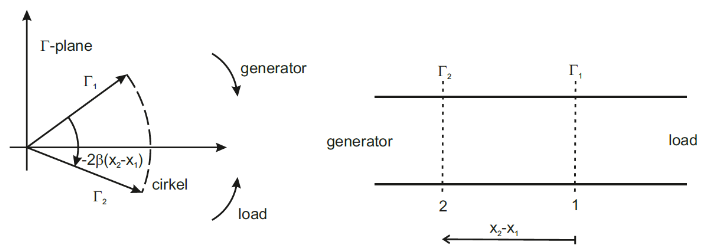
\includegraphics[width=0.8\linewidth]{../assets/chap03_prop2.png} %omg it contains the dutch 'cirkel' instead of 'circle', how did this book ever get published :|
					\caption{$\Gamma$ when moving on the transmission line}
					\label{fig:chap03_prop2}
				\end{figure}
				
			\subsubsection{Property 3}
				We normalize $Z_x$: $z_x = \frac{Z_x}{R_0}$. From here it follows that:
				\begin{equation}
					-\Gamma=\frac{y_x-1}{y_x+1}
				\end{equation}
				Here, $y_x = \frac{R_0}{Z_x} = \frac{Y_x}{G_0}$ is the normalized admittance. This means that we can find the admittance of a line easily on a smith chart by mirroring $\Gamma$ around the origin.
				
			\subsubsection{Property 4}
				In order to quickly go from $\Gamma$ to $z_x$ or vice versa, we must have curves of constant resistance and constant reactance in the $\Gamma$-plane (SD). We define short notation as follows:
				\begin{align}
					\Gamma &= u+jv\\
					z_x&=r+jx
				\end{align}
				Here, $r$ and $x$ are defined as:
				\begin{align}
					r=Re[z_x]=\frac{Re[Z_x]}{R_0}=\frac{R}{R_0}&\qquad\mathrm{resistance\ component}\\
					x=Im[z_x]=\frac{Im[Z_x]}{R_0}=\frac{X}{R_0}&\qquad\mathrm{reactance\ component}
				\end{align}
				These notations give way to the following equation:
				\begin{equation}
					\left[u-\frac{r}{1+r}\right]^2+v^2=\frac{1}{(1+r)^2} 
				\end{equation}
				This in the $(u,v)$-plane (SD) forms a circle for constant $r$ value. The radius of them is $\frac{1}{1+r}$ and the center is located at $\left(\frac{r}{1+r},0\right)$. These properties can be seen on figure \ref{fig:chap03_r-circles}.\\
				\\
				We also find 
				\begin{equation}
					[u-1]^2+\left[v-\frac{1}{2}\right]^2=\frac{1}{x^2}
				\end{equation}
				This gives a set of circles for constant $x$ in the $(u,v)$-plane. The radius is now $\left|\frac{1}{x}\right|$ and the center is $\left(1,\frac{1}{x}\right)$. These properties can be seen on figure \ref{fig:chap03_x-circles}.
				\begin{figure}[h]
					\centering
					\begin{subfigure}{.4\textwidth}
						\centering
						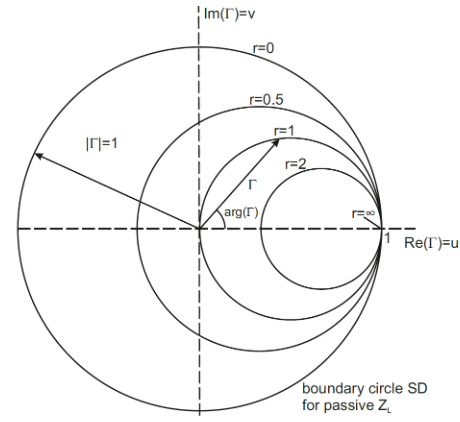
\includegraphics[width=1\linewidth]{../assets/chap03_r-circles.png} 
						\caption{Constant $r$-circles}
						\label{fig:chap03_r-circles}
					\end{subfigure}%
					\begin{subfigure}{.4\textwidth}
						\centering
						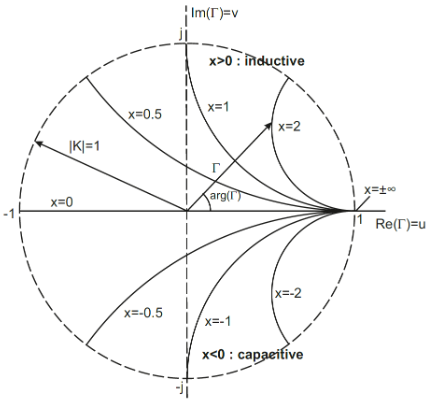
\includegraphics[width=1\linewidth]{../assets/chap03_x-circles.png} 
						\caption{Constant $x$-circles}
						\label{fig:chap03_x-circles}
					\end{subfigure}
					\caption{Two types of circles present on a Smith chart}
					\label{fig:circle_SD}
				\end{figure}\\
			
		\subsection{The smith chart itself}
			A proper smith chart is shown in figure \ref{fig:chap03_smith_chart} and examples of how to use it can be found in chapter three of the book from page 57 to 83. 
			\begin{figure}[h]
				\centering
				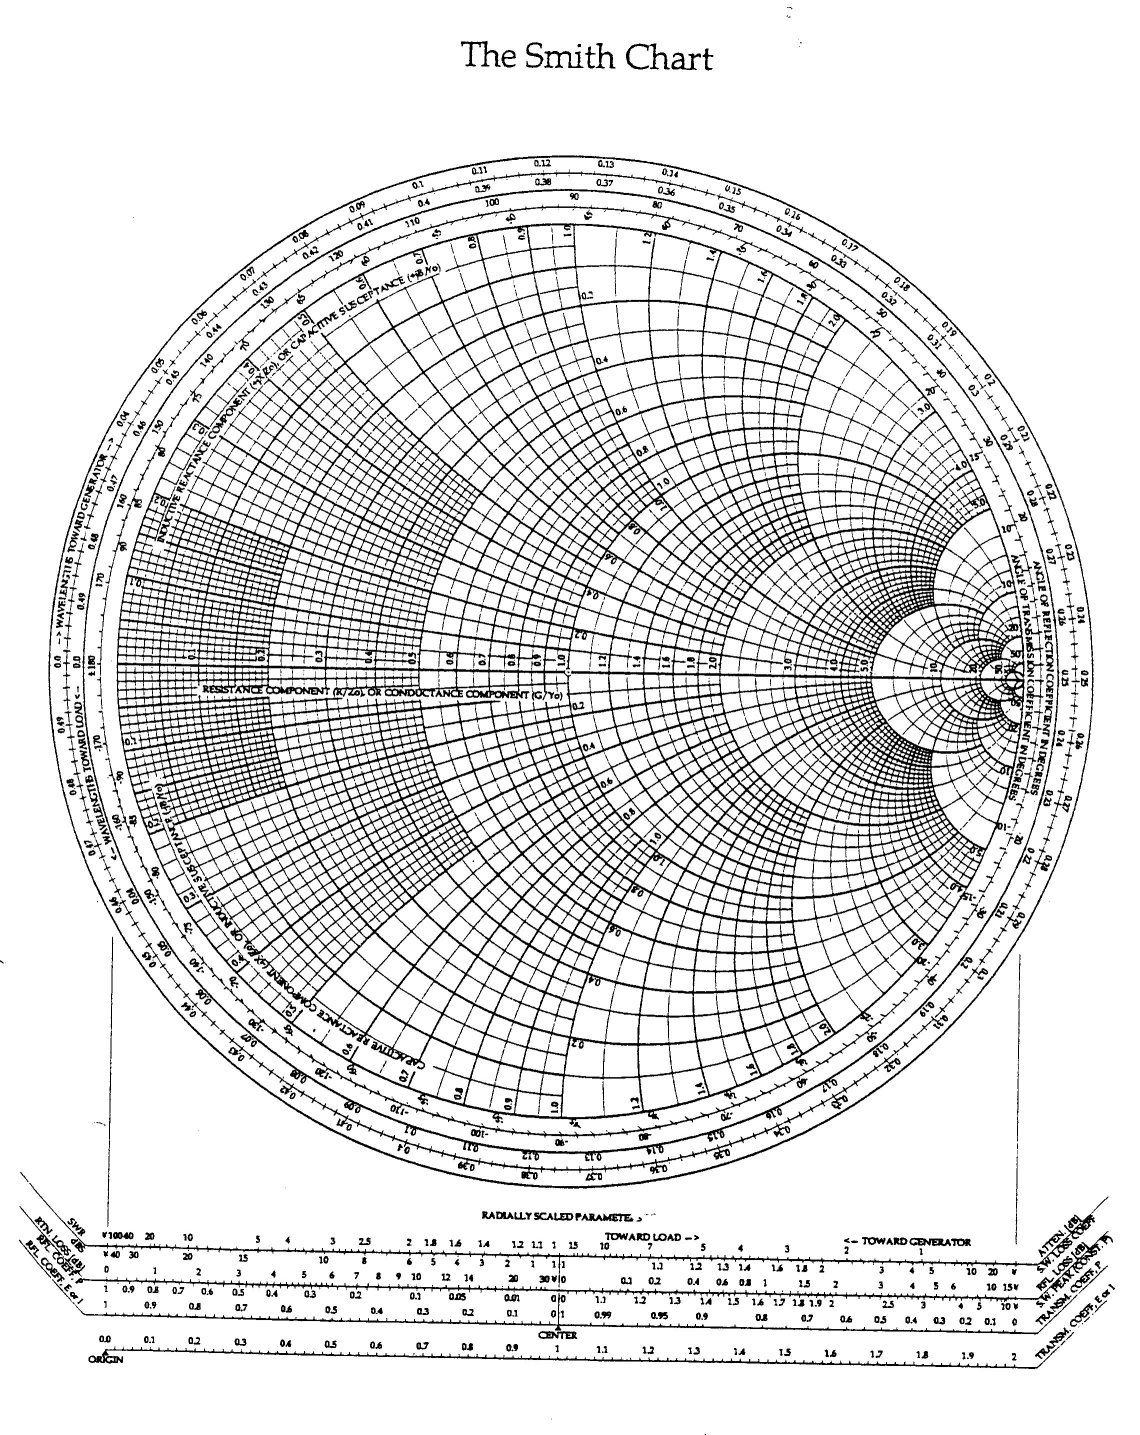
\includegraphics[width=1\linewidth]{../assets/chap03_smith_chart.jpg}
				\caption{A Smith chart}
				\label{fig:chap03_smith_chart}
			\end{figure}
\end{document}
